\subsection{Arquitectura de la aplicación}
\subsubsection{Servidor}
El servidor donde la aplicación iba a ser probada para su funcionamiento era
una máquina virtual GNU\\Linux que iba sobre una capa de
virtualización \gls{kvm}. Básicamente la empresa ya tenía \gls{kvm} montado y
simplemente tuve que configurar dicho servidor, adhiriéndome a los parámetros
que el informático de sistemas me facilitó.

\subsubsection{Sistema operativo}
El sistema operativo que escogí para montar el servidor fue Debian. El motivo
es que he utilizado mucho la susodicha distribución, y por lo tanto pensé que
sería mucho más fácil configurar una máquina utilizando una tecnología que ya
conocía. Debido a que en la empresa estaban de acuerdo con ello, fue finalmente
la que utilicé.

La distribución se clasifica principalmente en tres ramas: \textit{stable},
\textit{testing} y \textit{unstable}, y debido a que quería ahorrarme
quebraderos de cabeza en el futuro escogí la rama estable de la distribución.

No obstante, debido a su naturaleza estable, algunos de los paquetes que
requería \textemdash principalmente \gls{php} \textemdash no estaban en la
versión que ciertas librerías de la aplicación requerían, por lo que realicé
un pequeño ajuste con lo que se denomina \textit{apt-pinning}.

\textit{apt-pinning} se realiza cuando se precisa obtener versiones de
paquetes, o paquetes enteros, que no están en la rama de la distribución
actual. De esta forma se pueden obtener paquetes determinados en una versión
más moderna, permitiendo así tener las virtudes de un sistema en un estado
estable junto con las modernidades específicas de ciertos paquetes.

Esto se realizó después de comprobar que la primera opción recomendada,
los \gls{backports}{backports} para los paquetes necesarios, no estaban
disponibles por aquel momento.

\subsubsection{Base de datos}
Para la base de datos de la aplicación se utilizó \textit{MariaDB}, que es un
\glslink{fork}{fork} del proyecto de base de datos relacional \textit{MySQL}.
No se concibió utilizar una tecnología de base de datos diferente debido a
que no se esperaba que la aplicación fuera a gestionar un volumen y un tráfico
de datos que no fuera fácilmente manejable por una base de datos relacional. No
merecía la pena sacrificar ninguno de los principios \gls{acid}, ni tampoco un
\gls{rdbms} que proveyera del cumplimiento de los mismos, por una hipotética
necesidad de rendimiento y escalabilidad que fuera a requerir de un paradigma
de base de datos diferente.

El diagrama del \glslink{modentrel}{modelo entidad-relación} que usa la
aplicación se puede encontrar en la figura \ref{fig:erdiag}. La idea general es
que la aplicación podrá gestionar clientes, que a su vez agruparán proyectos
en grupos de proyectos. Cada proyecto puede categorizarse, y además puede tener
bolsas de horas \textemdash una especie de presupuesto en la que el cliente
consume horas de la susodicha bolsa de horas \textemdash y presupuestos. Los
proyectos predefinidos tienen como fin el ser una plantilla de la que copiar
los proyectos que son comunes a distintos grupos de proyectos. Los usuarios
pueden asignarse a proyectos, y además son los que crean las diferentes tareas
en cada proyecto. Las tareas favoritas tienen el mismo objetivo que los
proyectos predefinidos: facilitar la creación de tareas que se repiten
obteniéndolas de una lista previamente creada.

Este esquema se creó a raíz de las diferentes reuniones que se mantuvieron con
los interesados, en las cuales se debatió el modelo de gestión que tenían
decidido utilizar, y que dieron como fruto el esquema de la figura
\ref{fig:erdiag} que solventa y refleja las necesidades que se me expusieron.

Además, se puede observar que muchas de las entidades únicamente tienen un
par de campos: el identificador y el nombre. Esto es consecuencia de haber
consultado con los gestores sobre la adición de nuevos campos en las entidades,
que resultaran útiles para definir dichas entidades aún mejor. Pero en el
software que utilizaban no les daban un uso significativo, y tampoco preveían
que les fueran a dar más uso en esta aplicación. Por lo tanto decidí prescindir
de ellos e invertir el tiempo en otras tareas, pero manteniendo la estructura
del dominio de forma que si nuevos campos tuvieran que ser añadidos en el
futuro, algo que sí preveía probable, se pudiera hacer sin tener que
reestructurar el modelo.

\begin{figure}[p]
    \center
    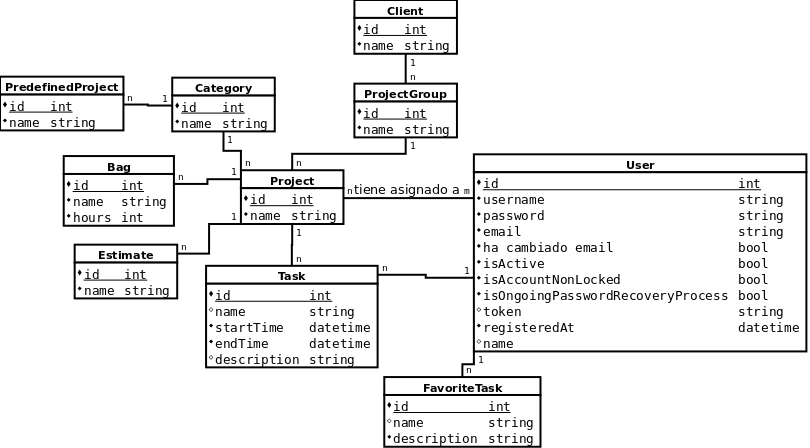
\includegraphics[angle=90,scale=0.6]{img/erDiagram}
    \caption{Diagrama del modelo entidad-relación de la base de
datos\label{fig:erdiag}}
\end{figure}

\subsubsection{Roles}
\label{sec:roles}
Por deseo de los interesados, los usuarios de la aplicación se iban a dividir
en tres grupos principales: gestor con privilegios, gestor, y usuario normal.
En la figura \ref{fig:useCases} se pueden apreciar los diferentes casos de uso
asignados a cada rol. También se puede observar que los roles se heredan, y por
lo tanto el gestor con privilegios heredará los casos de uso del gestor regular
y el usuario regular.

\begin{figure}[p]
    \center
    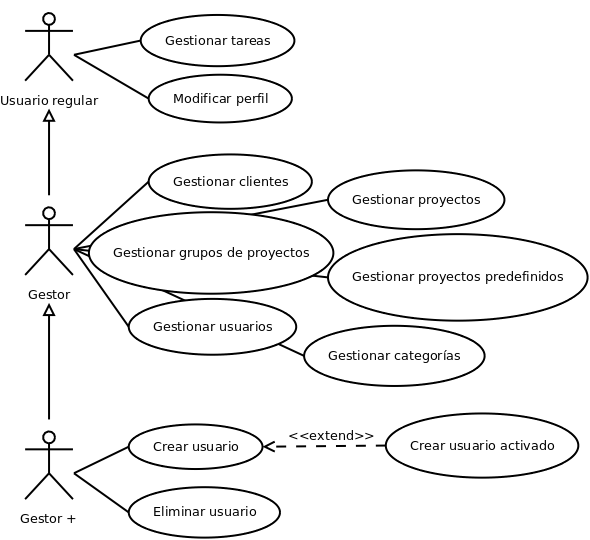
\includegraphics[scale=0.6]{img/useCase}
    \caption{Diagrama de casos de uso de la aplicación}
    \label{fig:useCases}
\end{figure}

\paragraph{Usuario regular}
El usuario con menos privilegios de la aplicación. La idea de este rol es que
los usuarios tengan la sensación de que sólo ellos están utilizando la
aplicación, y por lo tanto, se restringe el acceso a toda la información que no
tenga que ver directamente con él, y por lo tanto puede \textemdash por
gestionar se entiende crear, modificar y eliminar\textemdash:

\begin{itemize}
    \item Consultar su perfil de usuario.
    \item Modificar sus datos de usuario.
    \item Modificar su email y verificarlo.
    \item Modificar su contraseña.
    \item Recuperar la contraseña.
    \item Consultar los proyectos en los que toma parte \textemdash indicándole
        el nombre, grupo del proyecto y la categoría del mismo \textemdash.
    \item Gestionar tareas en los proyectos a los que está asignado.
    \item Gestionar sus tareas favoritas.
\end{itemize}

\paragraph{Gestor}
El gestor es el usuario con privilegios al que se le permite acceder y
modificar casi cualquier apartado de la aplicación. En la siguiente lista
se listan las funcionalidades a las que tiene acceso:

\begin{itemize}
    \item Gestionar clientes.
    \item Gestionar grupos de proyectos y asignarlos a clientes.
    \item Gestionar proyectos y asignarlos a grupos de proyectos, y también
        categorizarlos.
    \item Abrir y cerrar proyectos: de esta forma ningún usuario puede imputar
        más tareas al proyecto.
    \item Gestionar proyectos predefinidos. Además, los proyectos creados a
        partir de un proyecto predefinido verán sus campos modificados si un
        gestor modifica el proyecto predefinido al que está relacionado.
    \item Gestionar categorías.
    \item Gestionar bolsas de horas y asignarlas a proyectos.
    \item Gestionar presupuestos y asignarlos a proyectos.
    \item Gestionar las tareas de cualquier usuario de la aplicación.
    \item Gestionar las tareas favoritas de cualquier usuario de la aplicación.
    \item Modificar el perfil de cualquier usuario de la aplicación.
    \item Activar y desactivar un usuario, lo que permite restringirle por
        completo el acceso a la aplicación.
    \item Asignar y revocar el acceso de los usuarios a los proyectos.
\end{itemize}

\paragraph{Gestor con privilegios}
El gestor con privilegios es el usuario que puede utilizar la aplicación sin
ningún tipo de restricción. Los interesados del proyecto insistieron en que
únicamente un rol específico debería de poder añadir y eliminar usuarios de la
aplicación, ya que opinaban que eso facilitaría la gestión de la misma. Así que
las funcionalidades que se le ofrecen a los usuarios con este rol son:

\begin{itemize}
    \item Crear un usuario en la aplicación.
    \item Eliminar un usuario de la aplicación.
\end{itemize}
